\section{Visibility of a sub satellite point} 

 
\textbf{Let’s consider the point P on Earth located at \textit{P} (0° latitude, 0°, longitude). }
\begin{itemize}
    \item[-] \textbf{Describe (in plain language) the conditions for the point P to be visible from the CubeSat.}

    In general, many aspects need to be taken into consideration when determining a point's visibility from a satellite. 
    Most importantly, the point \textit{P} needs to be within \textit{Line of Sight} and inside the circular \textit{view factor area} of the satellite. 
    The CubeSat must have a clear and unobstructed line of sight to the point \textit{P}, which means that no part of Earth's surface should be blocking the view. 
    This can be analysed by means of the horizon distance, $D_H = \sqrt{2\, R_E\,h}$, which forms a triangle between the satellite, the point in the horizon and Earth's centre. 
    By looking at the maximum case of the triangle, we can determine a trigonometric relationship and find the maximum angle, $\alpha$, in both latitude and longitude:
    
    \begin{equation}
        \label{eq:max_angle}
        \begin{split}
            \alpha &= arcsin \left(\frac{D_H}{R_e + h}\right) \\
            &= arcsin \left(\frac{\sqrt{2\, R_E\,h}}{R_e + h}\right) \qquad || R_E = 6378\,km, \, h = 408\,km \\
            &= 19.644385\text{°} \approx 19.6\text{°}
        \end{split}
    \end{equation}

    In other words, for a point \textit{P} to be visible from the satellite, the satellite's footprint needs to be between $-19.6$° and $19.6$° in both longitude and latitude.


    The \textit{Orbital Path and Period} thus play a vital role in the visibility of point \textit{P}. 
    The orbital path must be such that it brings the satellite into line of sight with the point \textit{P}. 
    E.g. very high inclination orbits, such as polar orbits, or geostationary orbits could be obtained in such a way that the point \textit{P} would never be visible.
    Since the CubeSat has a circular orbit and an inclination of 51,6°, it will travel between 51.6° North and 51.6° South, crossing the equator in between. 
    This means that at some points during its orbits, the satellite will cross over the point \textit{P} (between $-19.6$° and $19.6$° in both longitude and latitude).
    \autoref{fig:null} shows a Molniya orbit and the real-world location of the point \textit{P}.
    
    \begin{figure}[H]
        \centering
        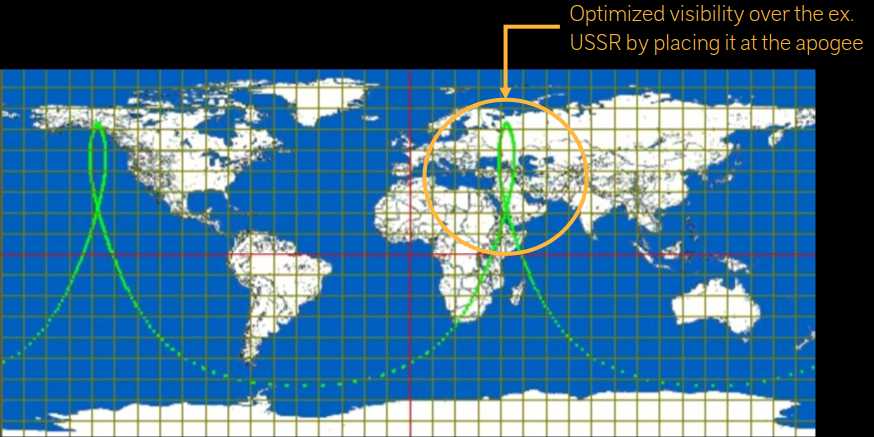
\includegraphics[width=0.75\linewidth]{Doc//Graphics/Molniya.png}
        \caption{Groundtrack of a Molniya orbit. The equator and prime meridian intersect at Null island (in red).}
        \label{fig:null}
    \end{figure}    

    Realistically, \textit{Night and Day visibility} would also play a role. 
    While technically the point would be visible as long as the Line of Sight requirement is met, it is also important to remember in real-life applications that the point \textit{P} might not be visible to the CubeSat during night-time when it is dark.
    Depending on the instruments onboard the CubeSat and what is meant by "visible", i.e. visible to a communications array or visible in the sense that the satellite can take a clear image of the point \textit{P}.
    With the given orbital parameters, and an assumed orbital speed similar to the ISS (7.66 km/s), the CubeSat's orbital period would be about 92 min, meaning that it completes a whole orbit around Earth every 92 minutes. 
    As such, it would pass over the equator often enough that it would intersect with daytime.
    




    \newpage
    \item[-] \textbf{Describe an algorithm that allows to determine if the point P is visible from the CubeSat. } 

    For point \textit{P} to be visible from the satellite, the norm of the vector between \textit{P} and the satellite footprint point $P_f$ coordinates needs to be smaller or equal to the norm of a vector between \textit{P} and $P_{max}$ (19.7°, 19.7°).
    This can be mathematically expressed as below:
    \begin{equation}
        \label{eq:p_visible}
        \begin{split}
            \sqrt{P_{f,lat}^2 + P_{f,long}^2} &\leq \sqrt{P_{max,lat}^2 + P_{max,long}^2} \\
            \sqrt{P_{f,lat}^2 + P_{f,long}^2} &\leq \sqrt{(19.7^\circ)^2 + (19.7^\circ)^2}
        \end{split}
    \end{equation}
    
    \item[-] \textbf{Code this algorithm and show, on a ground map, the points of the orbit which are visible from this point P.}

    Somethin \autoref{sec:Appendix_A} on lines XX using the \verb|...| function and the output plot can be seen below in \autoref{fig:}.
    

    
    \item[-] \textbf{What is the duration of the visibility for a satellite passing at the zenith of P?}
\end{itemize}

 
\vspace{0.5cm}
\begin{itemize}
    \item[-] \textbf{Express the vector (CubeSat, P) in satellite local orbital frame.}
    \item[-] \textbf{Describe an algorithm to compute the direction of the point P in local orbital reference frame.}
    \item[-] Code this algorithm and show, on a 3D plot, the vector wrt time over one orbit.
\end{itemize}